\section{Background}
\label{background}

The World-Wide Web (WWW), commonly known as the web, was invented to ''to be a pool of human knowledge'' \parencite*[76]{BernersLeeCailliauLuotonenNielsenSecret1994} that could be shared between remote collaborators \parencite{BernersLeeCailliauLuotonenNielsenSecret1994}. HyperText Markup Language (HTML), Cascading Style Sheets (CSS), and JavaScript (JS) are considered the core web technologies \parencite{MajchrzakBiornHansenGronli2018}. The core web technologies that are all being used today were all introduced in just a few years in 1993 to 1996 (Figure \ref{webtechnologies-timeline}).

\begin{figure}[!h]
\centering
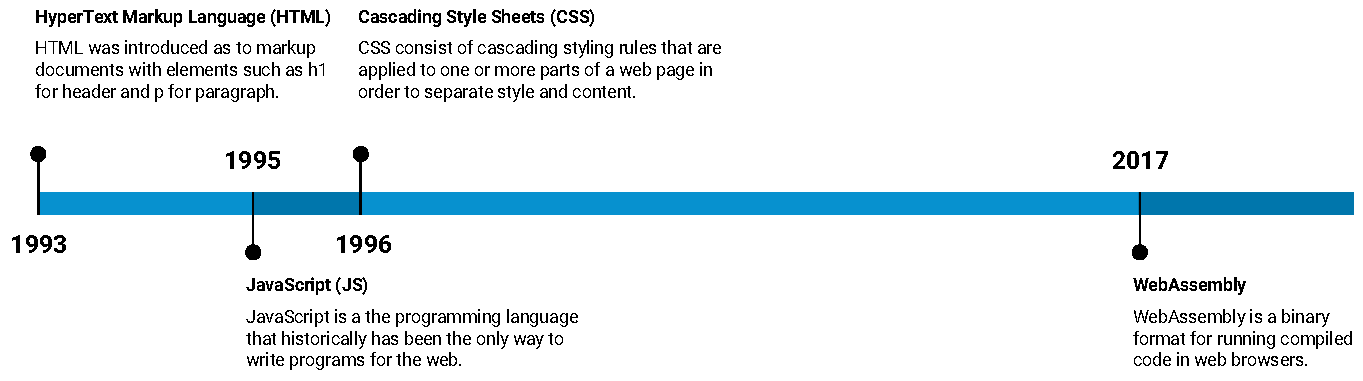
\includegraphics[width=16cm,keepaspectratio]{../Figures/webtechnologies-timeline}
\caption{Timeline of major web technologies: HTML, CSS, JavaScript and it's newest member WebAssembly.}
\label{webtechnologies-timeline}
\end{figure}

The very first web page (Figure \ref{world-wide-web}) was written in HTML and relies heavily on hyperlinks \parencite{BernersLeeCailliauGroffPollermann1992}. In 1996 the W3C recommendation on CSS was published \parencite{LieBos1996}. \citeauthor{LieBos1996} describes CSS as a simple mechanism that ''allows authors and readers to attach style (e.g. fonts, colors and spacing) to HTML documents'' \parencite*[1]{LieBos1996} based on CSS rules. JavaScript was introduced in 1995 intended to be used for simple tasks such as client-side form validation or simple animations \parencite{Moller2018}. It's capabilities evolved and led to inventions such as Asynchronous JavaScript and XML (AJAX) \parencite{NielsonWilliamsonArlitt2008} and heavy manipulation of the Document Object Model (DOM) \parencite{WoodLeHorsApparaoByrneChampionIsaacsJacobsNicolRobieSutor1998}.

%The number of web pages published on the web grew fast. According to \textcite{BrinPage1998} World Wide Web Worm, one of the first search engines, had in 1994 110,000 pages in it's index. In 1997 the index of the top search engines at that time contained at least 2 million web pages \parencite{BrinPage1998}.

%\hl{how about today?} Today there are more than 1 billion web \emph{sites} on the web \hl{ref}, where each site contains at least one page, normally many many more. \hl{the definition of a page is no longer clear}. As will be described in the chapter on web apps the definition of a page is no longer an easy one to make.

% The core web technologies HTML, CSS and JavaScript has the been the same since the first half of 1990. They were invented for researchers to share documents with each other, but thas the last few years become incresingly popular as the underpining of web applications. The major enabler for web applications is JavaScript, which has since it was introduced in Netscape Navigator in 1995 been the only way to write program that could be interpreted by web browsers.

% The last few years more advanced applications has moved to the web, mandating higher performance (REF).

% dynamiska webbsidor typ som första kapitel och att de i många fall lider av prestandaproblem, sätter upp varför vi behöver benchmarking.

\begin{figure}[!h]
\centering
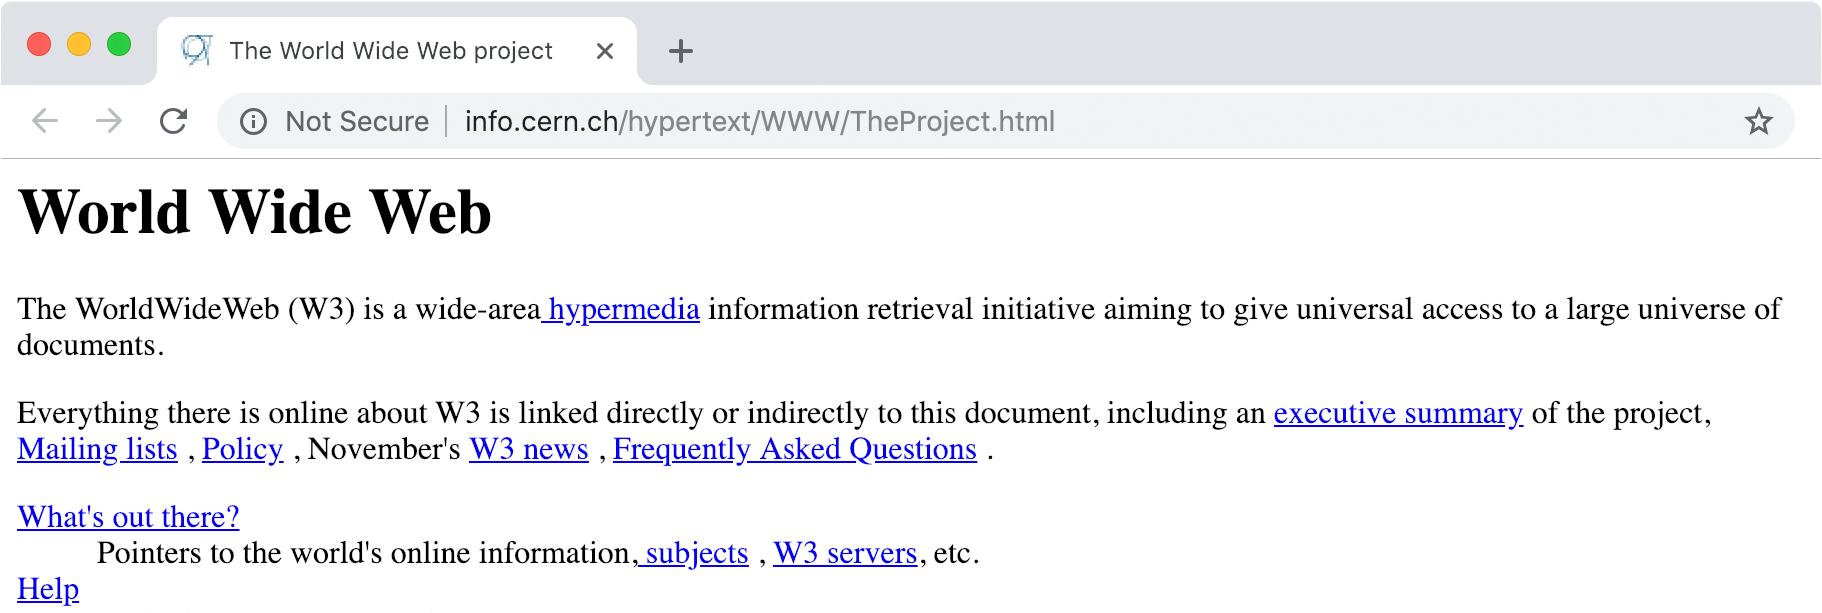
\includegraphics[width=16cm,keepaspectratio]{../Figures/world-wide-web}
\caption{The first web page created by Tim Berners-Lee.}
\label{world-wide-web}
\end{figure}

The introduction and evoluation of JavaScript has lead the evolution of the web browser as a web page reader towards a platform for web applications.

\subsection{Web apps}
\subfile{webapps}

\subsection{JavaScript}
\subfile{javascript}

\subsection{WebAssembly}
\subfile{webassembly}

\subsection{Benchmarking}
\subfile{benchmarking}
